% Options for packages loaded elsewhere
\PassOptionsToPackage{unicode}{hyperref}
\PassOptionsToPackage{hyphens}{url}
\PassOptionsToPackage{dvipsnames,svgnames,x11names}{xcolor}
%
\documentclass[
  letterpaper,
  DIV=11,
  numbers=noendperiod]{scrartcl}

\usepackage{amsmath,amssymb}
\usepackage{lmodern}
\usepackage{iftex}
\ifPDFTeX
  \usepackage[T1]{fontenc}
  \usepackage[utf8]{inputenc}
  \usepackage{textcomp} % provide euro and other symbols
\else % if luatex or xetex
  \usepackage{unicode-math}
  \defaultfontfeatures{Scale=MatchLowercase}
  \defaultfontfeatures[\rmfamily]{Ligatures=TeX,Scale=1}
\fi
% Use upquote if available, for straight quotes in verbatim environments
\IfFileExists{upquote.sty}{\usepackage{upquote}}{}
\IfFileExists{microtype.sty}{% use microtype if available
  \usepackage[]{microtype}
  \UseMicrotypeSet[protrusion]{basicmath} % disable protrusion for tt fonts
}{}
\makeatletter
\@ifundefined{KOMAClassName}{% if non-KOMA class
  \IfFileExists{parskip.sty}{%
    \usepackage{parskip}
  }{% else
    \setlength{\parindent}{0pt}
    \setlength{\parskip}{6pt plus 2pt minus 1pt}}
}{% if KOMA class
  \KOMAoptions{parskip=half}}
\makeatother
\usepackage{xcolor}
\setlength{\emergencystretch}{3em} % prevent overfull lines
\setcounter{secnumdepth}{-\maxdimen} % remove section numbering
% Make \paragraph and \subparagraph free-standing
\ifx\paragraph\undefined\else
  \let\oldparagraph\paragraph
  \renewcommand{\paragraph}[1]{\oldparagraph{#1}\mbox{}}
\fi
\ifx\subparagraph\undefined\else
  \let\oldsubparagraph\subparagraph
  \renewcommand{\subparagraph}[1]{\oldsubparagraph{#1}\mbox{}}
\fi


\providecommand{\tightlist}{%
  \setlength{\itemsep}{0pt}\setlength{\parskip}{0pt}}\usepackage{longtable,booktabs,array}
\usepackage{calc} % for calculating minipage widths
% Correct order of tables after \paragraph or \subparagraph
\usepackage{etoolbox}
\makeatletter
\patchcmd\longtable{\par}{\if@noskipsec\mbox{}\fi\par}{}{}
\makeatother
% Allow footnotes in longtable head/foot
\IfFileExists{footnotehyper.sty}{\usepackage{footnotehyper}}{\usepackage{footnote}}
\makesavenoteenv{longtable}
\usepackage{graphicx}
\makeatletter
\def\maxwidth{\ifdim\Gin@nat@width>\linewidth\linewidth\else\Gin@nat@width\fi}
\def\maxheight{\ifdim\Gin@nat@height>\textheight\textheight\else\Gin@nat@height\fi}
\makeatother
% Scale images if necessary, so that they will not overflow the page
% margins by default, and it is still possible to overwrite the defaults
% using explicit options in \includegraphics[width, height, ...]{}
\setkeys{Gin}{width=\maxwidth,height=\maxheight,keepaspectratio}
% Set default figure placement to htbp
\makeatletter
\def\fps@figure{htbp}
\makeatother
\newlength{\cslhangindent}
\setlength{\cslhangindent}{1.5em}
\newlength{\csllabelwidth}
\setlength{\csllabelwidth}{3em}
\newlength{\cslentryspacingunit} % times entry-spacing
\setlength{\cslentryspacingunit}{\parskip}
\newenvironment{CSLReferences}[2] % #1 hanging-ident, #2 entry spacing
 {% don't indent paragraphs
  \setlength{\parindent}{0pt}
  % turn on hanging indent if param 1 is 1
  \ifodd #1
  \let\oldpar\par
  \def\par{\hangindent=\cslhangindent\oldpar}
  \fi
  % set entry spacing
  \setlength{\parskip}{#2\cslentryspacingunit}
 }%
 {}
\usepackage{calc}
\newcommand{\CSLBlock}[1]{#1\hfill\break}
\newcommand{\CSLLeftMargin}[1]{\parbox[t]{\csllabelwidth}{#1}}
\newcommand{\CSLRightInline}[1]{\parbox[t]{\linewidth - \csllabelwidth}{#1}\break}
\newcommand{\CSLIndent}[1]{\hspace{\cslhangindent}#1}

\KOMAoption{captions}{tableheading}
\makeatletter
\makeatother
\makeatletter
\makeatother
\makeatletter
\@ifpackageloaded{caption}{}{\usepackage{caption}}
\AtBeginDocument{%
\ifdefined\contentsname
  \renewcommand*\contentsname{Table of contents}
\else
  \newcommand\contentsname{Table of contents}
\fi
\ifdefined\listfigurename
  \renewcommand*\listfigurename{List of Figures}
\else
  \newcommand\listfigurename{List of Figures}
\fi
\ifdefined\listtablename
  \renewcommand*\listtablename{List of Tables}
\else
  \newcommand\listtablename{List of Tables}
\fi
\ifdefined\figurename
  \renewcommand*\figurename{Figure}
\else
  \newcommand\figurename{Figure}
\fi
\ifdefined\tablename
  \renewcommand*\tablename{Table}
\else
  \newcommand\tablename{Table}
\fi
}
\@ifpackageloaded{float}{}{\usepackage{float}}
\floatstyle{ruled}
\@ifundefined{c@chapter}{\newfloat{codelisting}{h}{lop}}{\newfloat{codelisting}{h}{lop}[chapter]}
\floatname{codelisting}{Listing}
\newcommand*\listoflistings{\listof{codelisting}{List of Listings}}
\makeatother
\makeatletter
\@ifpackageloaded{caption}{}{\usepackage{caption}}
\@ifpackageloaded{subcaption}{}{\usepackage{subcaption}}
\makeatother
\makeatletter
\@ifpackageloaded{tcolorbox}{}{\usepackage[many]{tcolorbox}}
\makeatother
\makeatletter
\@ifundefined{shadecolor}{\definecolor{shadecolor}{rgb}{.97, .97, .97}}
\makeatother
\makeatletter
\makeatother
\ifLuaTeX
  \usepackage{selnolig}  % disable illegal ligatures
\fi
\IfFileExists{bookmark.sty}{\usepackage{bookmark}}{\usepackage{hyperref}}
\IfFileExists{xurl.sty}{\usepackage{xurl}}{} % add URL line breaks if available
\urlstyle{same} % disable monospaced font for URLs
\hypersetup{
  pdftitle={Assignment-5},
  pdfauthor={Frøydis Gretteberg},
  colorlinks=true,
  linkcolor={blue},
  filecolor={Maroon},
  citecolor={Blue},
  urlcolor={Blue},
  pdfcreator={LaTeX via pandoc}}

\title{Assignment-5}
\author{Frøydis Gretteberg}
\date{}

\begin{document}
\maketitle
\ifdefined\Shaded\renewenvironment{Shaded}{\begin{tcolorbox}[interior hidden, borderline west={3pt}{0pt}{shadecolor}, enhanced, boxrule=0pt, breakable, sharp corners, frame hidden]}{\end{tcolorbox}}\fi

\hypertarget{introduksjon}{%
\subsection{Introduksjon}\label{introduksjon}}

Treningsvolum og muskelstyrke er et mye omdiskutert felt, som det har
blitt gjort mye forskning på. Felles for mye av de tidligere studiene på
dette feltet er at de har fått ganske like resultater {[}SCHOENFELD et
al. (2019){]}(HASS et al. 2000)(Heaselgrave et al. 2019). Disse
resultatene har vist en signifikant økning i muskelhypertrofi blant
mennesker i ulike grupper med bare et lavt styrketreningsvolum. Det vil
si at det skjer en muskeløkning for både trente og utrente personer når
de øker styrketreningsvolum.

Videre har forskningen også vist at det er en lite til ingen signifikant
forskjell mellom de som trener ett sett med 8-12 repetisjoner og de som
trener tre sett med like mange repetisjoner, men at det mest optimale er
å ligge midt i mellom (Aube et al. 2020).

For å oppnå muskelhypertrofi, økning i muskelcellenes størrelse, blir
styrketrening ansett som den mest effektive treningsformen (Souza,
Barbalho, and Gentil 2020). Selv om det er en enighet at styrketrening
er den beste formen for muskelhypertrofi er det fortsatt flere faktorer
som kan påvirke muskelvekst. Faktorer som hvilken type styrketrening,
volum, frekvens og intensitet kan påvirke muskelvekst (Souza, Barbalho,
and Gentil 2020)

I denne studien vil formålet være å se hvordan singel sett eller flere
sett (tre sett) kan være en påvirkningsfaktor for muskelhypertrofi.

\hypertarget{section}{%
\subsection{}\label{section}}

Metode

\hypertarget{deltakere-og-studieoversikt}{%
\subsubsection{Deltakere og
studieoversikt}\label{deltakere-og-studieoversikt}}

I denne studien var det 41 deltakere som ble rekruttert, og utvalget
besto av både kvinner og menn. Alderen på deltakerne varierte fra 18-40
år. For selektering av utvalg ble det brukt inklusjonskriteriet og
eksklusjonskriterier. Hovedkriteriene var at deltakerne måtte være
ikke-røykere, de skulle ikke ha en intoleranse mot lokalbedøvelse,
deretter ble treningshistorikk, eventuelle skader og medisiner brukt som
ekskludering. Hvis noen av de overnevnte faktorene kunne påvirke
styrketreningen ble deltakerne ekskludert. Underveis i studien ble hele
syv deltakere utelukket, da de ikke oppfylte kravet om 85\% deltakelse.
Alle som deltok på studien hadde historikk fra sportslige aktiviteter,
dette var dog ikke et kriterium.

Selve intervensjonen besto av 12 uker med fullkroppsstyrketrening. For
målinger ble det utført muskelbiopsi i vastus lateralis før
intervensjonen, i uke 2 og etter endt intervensjon. Muskelstyrke ble
også målt ved baseline og ved endt intervensjon. På baseline var lite
til ingen signifikant forskjell mellom de ulike gruppene som kunne vært
en fordel eller ulempe i testen. Beinøvelsene som ble gjennomført under
intervensjonen ble utført på hvert ben, dette for å kunne muliggjøre
individuelle forskjeller i treningsvolum. Deltakerne fikk tilfeldig
utdelt om de skulle gjennomføre ett sett eller multiple sett.

MRI-scan ble brukt både før og etter intervensjonen for å måle
tversnittarealet til musklene i quadricepsgruppen (vastus lateralis,
medialis, intermedius og rectus femoris). DXA-scan ble brukt for å måle
kroppssammensetningen. Deltakeren måtte være fastende i 2 timer før både
MRI-scan og DXA-scan, og unngå all form for hard fysisk aktivitet i 48
timer før.

\hypertarget{treningsprotokoller}{%
\subsubsection{Treningsprotokoller}\label{treningsprotokoller}}

For standardisering ble det laget et universelt oppvarmingsprogram.
Dette programmet inneholdt 5 minutter med sykling, etterfulgt med 10
repetisjoner av øvelsene: pushups, situps, rygghev og knebøy. Alle
øvelser ble utført med egen kroppsvekt. For de øvelsene som også var en
del av intervensjonen ble de utført ekstra 10 repetisjoner med 50\% vekt
av 1RM.

Videre for standarisering ble alle beinøvelser utført med en gitt
rekkefølge: beinpress, knefleksjon etterfulgt av kneekstensjon. Videre
ble øvelsene bilateral benkpress, nedtrekk, skulderpress eller sittende
roing implementert i programmet etter beinøvelsene. Mellom hver øvelse
var det en pause på mellom 90-180 sekunder. For progresjon ble
intensiteten økt underveis i intervensjonen.

1RM ble brukt for å beskrive maksimal styrke i beinpress og
kneekstensjon. 1RM fant de etter progressiv økning av motstanden slik at
deltakeren ikke klarte å løfte vekten mer. Alle deltakere fikk mellom
4-6 forsøk, med restitusjonstid mellom hvert sett. ~

Mellom hver treningsøkt var det en pause på minst 48 timer når det hadde
vært en økt med maksimal intensitet og 24 timer mellom hver økt med
submaksimal styrke. For å starte restitusjonen fikk deltakerne tildelt
en standardisert drikke etter hver øvelse.

\hypertarget{analysestatistikk}{%
\subsection{Analyse/Statistikk}\label{analysestatistikk}}

Med mindre annet er beskrevet er all deskriptiv data presentert som et
gjennomsnitt og standardavvik. For å måle effekten av antall sett
(treningsvolum) på muskelhypertrofi og muskelstyrke ble det brukt
lineære modeller. P-verdier er regnet ut ved hjelp av ANCOA-modell.
Statistisk signifikans ble satt til α=0,05.

\hypertarget{resultater}{%
\subsection{Resultater}\label{resultater}}

Totalt førte den 12 uker lange intervensjonen i denne studien, med
planlagt styrketrening, til en signifikant økning i muskelstyrke.
Økningen hadde henholdsvis 31±14\% single sett og 25±13\% for multiple
sett, noe som gir en P-verdi på (P\textbackslash\textless0,001).
Økningen i muskelvekst var også signifikant, på hele 2±4 for single sett
og 3,3±4\% for multiple sett (P\textbackslash\textless0,001).

\hypertarget{muskelvekst-pre--og-posttest}{%
\subsubsection{Muskelvekst pre- og
posttest}\label{muskelvekst-pre--og-posttest}}

\begin{figure}

{\centering 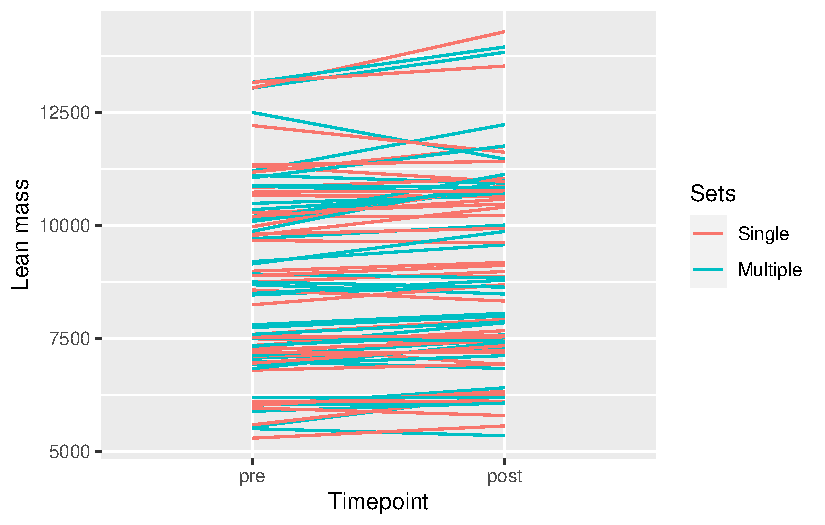
\includegraphics{Assignment-5-_files/figure-pdf/unnamed-chunk-1-1.pdf}

}

\caption{Figure 1: Change in lean mass from pre to post, single
vs.~multiple sets}

\end{figure}

\hypertarget{maksimal-muskelstyrke}{%
\subsubsection{Maksimal muskelstyrke}\label{maksimal-muskelstyrke}}

\begin{figure}

{\centering 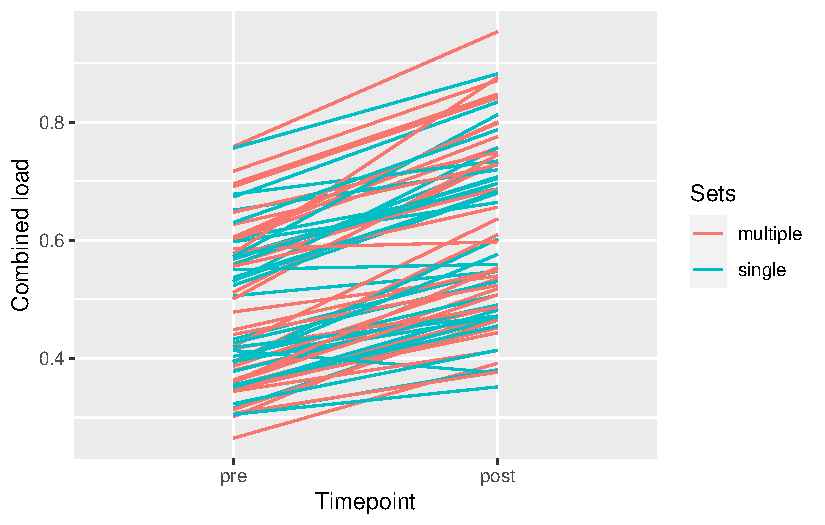
\includegraphics{Assignment-5-_files/figure-pdf/unnamed-chunk-3-1.pdf}

}

\caption{Figure 2: Change in strength (combined load) from pre to post,
single vs.~multiple sets}

\end{figure}

\hypertarget{diskusjon}{%
\subsection{Diskusjon}\label{diskusjon}}

I denne studien var det en større økning i muskelstyrke og muskelvekst
fra pre- til posttest blant de som trente multiple sett enn de som
trente single sett. Derimot ser vi også i figur 2 at både de som har
trent med single sett og multiple sett har hatt en økning. Dette kan
støttes av Hass et al.~(2000) som også så en økning i muskelstyrke og
muskelvekst i både singel- og multiple sett(HASS et al. 2000).

\hypertarget{refs}{}
\begin{CSLReferences}{1}{0}
\leavevmode\vadjust pre{\hypertarget{ref-aube2020}{}}%
Aube, Daniel, Tanuj Wadhi, Jacob Rauch, Ashmeet Anand, Christopher
Barakat, Jeremy Pearson, Joshua Bradshaw, Spencer Zazzo, Carlos
Ugrinowitsch, and Eduardo O. De Souza. 2020. {``Progressive Resistance
Training Volume: Effects on Muscle Thickness, Mass, and Strength
Adaptations in Resistance-Trained Individuals.''} \emph{Journal of
Strength and Conditioning Research} 36 (3): 600--607.
\url{https://doi.org/10.1519/jsc.0000000000003524}.

\leavevmode\vadjust pre{\hypertarget{ref-hass2000}{}}%
HASS, CHRIS J., LINDA GARZARELLA, DIEGO DE HOYOS, and MICHAEL L.
POLLOCK. 2000. {``Single Versus Multiple Sets in Long-Term Recreational
Weightlifters.''} \emph{Medicine \& Science in Sports \& Exercise},
January, 235. \url{https://doi.org/10.1097/00005768-200001000-00035}.

\leavevmode\vadjust pre{\hypertarget{ref-heaselgrave2019}{}}%
Heaselgrave, Samuel R., Joe Blacker, Benoit Smeuninx, James McKendry,
and Leigh Breen. 2019. {``Dose-Response Relationship of Weekly
Resistance-Training Volume and Frequency on Muscular Adaptations in
Trained Men.''} \emph{International Journal of Sports Physiology and
Performance} 14 (3): 360--68.
\url{https://doi.org/10.1123/ijspp.2018-0427}.

\leavevmode\vadjust pre{\hypertarget{ref-schoenfeld2019}{}}%
SCHOENFELD, BRAD J., BRET CONTRERAS, JAMES KRIEGER, JOZO GRGIC, KENNETH
DELCASTILLO, RAMON BELLIARD, and ANDREW ALTO. 2019. {``Resistance
Training Volume Enhances Muscle Hypertrophy but Not Strength in Trained
Men.''} \emph{Medicine \& Science in Sports \& Exercise} 51 (1):
94--103. \url{https://doi.org/10.1249/mss.0000000000001764}.

\leavevmode\vadjust pre{\hypertarget{ref-souza2020}{}}%
Souza, Daniel, Matheus Barbalho, and Paulo Gentil. 2020. {``The Impact
of Resistance Training Volume on Muscle Size and Lean Body Mass: To
Infinity and Beyond?''} \emph{Human Movement} 21 (4): 18--29.
\url{https://doi.org/10.5114/hm.2020.94199}.

\end{CSLReferences}



\end{document}
